%%%%%%%%%%%%%%%%%%%%%%%%%%%%%%%%%%%%%%%%%
% Masters/Doctoral Thesis
% LaTeX Template
% Version 2.5 (27/8/17)
%
% This template was downloaded from:
% http://www.LaTeXTemplates.com
%
% Version 2.x major modifications by:
% Vel (vel@latextemplates.com)
%
% This template is based on a template by:
% Steve Gunn (http://users.ecs.soton.ac.uk/srg/softwaretools/document/templates/)
% Sunil Patel (http://www.sunilpatel.co.uk/thesis-template/)
%
% Template license:
% CC BY-NC-SA 3.0 (http://creativecommons.org/licenses/by-nc-sa/3.0/)
%
%%%%%%%%%%%%%%%%%%%%%%%%%%%%%%%%%%%%%%%%%

%----------------------------------------------------------------------------------------
%	PACKAGES AND OTHER DOCUMENT CONFIGURATIONS
%----------------------------------------------------------------------------------------

\documentclass[
11pt, french, % The default document font size, options: 10pt, 11pt, 12pt
oneside, % Two side (alternating margins) for binding by default, uncomment to switch to one side
% english, % ngerman for German
singlespacing, % Single line spacing, alternatives: onehalfspacing or doublespacing
%draft, % Uncomment to enable draft mode (no pictures, no links, overfull hboxes indicated)
%nolistspacing, % If the document is onehalfspacing or doublespacing, uncomment this to set spacing in lists to single
%liststotoc, % Uncomment to add the list of figures/tables/etc to the table of contents
%toctotoc, % Uncomment to add the main table of contents to the table of contents
% parskip, % Uncomment to add space between paragraphs
%nohyperref, % Uncomment to not load the hyperref package
headsepline, % Uncomment to get a line under the header
chapterinoneline, % Uncomment to place the chapter title next to the number on one line
%consistentlayout, % Uncomment to change the layout of the declaration, abstract and acknowledgements pages to match the default layout
]{MastersDoctoralThesis} % The class file specifying the document structure

\usepackage[utf8]{inputenc} % Required for inputting international characters
\usepackage[T1]{fontenc} % Output font encoding for international characters
\usepackage{mathpazo} % Use the Palatino font by default
\usepackage[backend=bibtex,natbib=true]{biblatex} % Use the bibtex backend with the authoryear citation style (which resembles APA)
\usepackage{listings}
\usepackage[autostyle=true]{csquotes}

\addbibresource{rapport.bib} % The filename of the bibliography

\usepackage[autostyle=true]{csquotes} % Required to generate language-dependent quotes in the bibliography

%----------------------------------------------------------------------------------------
%	MARGIN SETTINGS
%----------------------------------------------------------------------------------------

\geometry{
	paper=a4paper, % Change to letterpaper for US letter
	inner=2.5cm, % Inner margin
	outer=3.8cm, % Outer margin
	bindingoffset=.5cm, % Binding offset
	top=1.5cm, % Top margin
	bottom=1.5cm, % Bottom margin
	%showframe, % Uncomment to show how the type block is set on the page
}

%----------------------------------------------------------------------------------------
%	THESIS INFORMATION
%----------------------------------------------------------------------------------------

\thesistitle{Étude de l'impact de l'utilisation des IA génératives de code sur les developpeurs}
\supervisor{Jean-Rémy FALLERI}
\author{Maxime \textsc{PICO}}

\subject{Biological Sciences}
\keywords{}
\university{\href{https://www.u-bordeaux.fr}{Université de Bordeaux}}
\department{\href{http://www.labri.fr}{LaBRI}}
\group{\href{https://www.labri.fr/programmation-reseaux-et-systemes}{Groupe Progress}}
\faculty{}

\AtBeginDocument{
\hypersetup{pdftitle=\ttitle} % Set the PDF's title to your title
\hypersetup{pdfauthor=\authorname} % Set the PDF's author to your name
\hypersetup{pdfkeywords=\keywordnames} % Set the PDF's keywords to your keywords
}

\begin{document}

\frontmatter % Use roman page numbering style (i, ii, iii, iv...) for the pre-content pages

\pagestyle{plain} % Default to the plain heading style until the thesis style is called for the body content

%----------------------------------------------------------------------------------------
%	TITLE PAGE
%----------------------------------------------------------------------------------------

\begin{titlepage}
\begin{center}

\vspace*{.06\textheight}
{\scshape\LARGE \univname\par}\vspace{1.5cm} % University name
% \vspace*{.06\textheight}
% \vspace*{\fill}
% {
%   % \scshape\LARGE
%   \raisebox{-0.5\height}{\includegraphics[scale=1, height=1.7cm]{images/brdx.pdf}}
%   \hspace{4cm}
%   \raisebox{-0.5\height}{
\includegraphics[scale=1, height=0.8cm]{images/labri.png}}
%   \par
%   %\univname\par
% }\vspace{1.5cm} % University name
\textsc{\Large Rapport de Stage}\\[0.5cm] % Thesis type

\HRule \\[0.4cm] % Horizontal line
{\huge \bfseries \ttitle\par}\vspace{0.4cm} % Thesis title
\HRule \\[1.5cm] % Horizontal line

\begin{minipage}[t]{0.4\textwidth}
\begin{flushleft} \large
\emph{Auteur:}\\
\authorname
%\href{http://www.johnsmith.com}{\authorname}
\end{flushleft}
\end{minipage}
\begin{minipage}[t]{0.4\textwidth}
\begin{flushright} \large
\emph{Encadrant:} \\
\href{https://www.labri.fr/perso/falleri/}{\supname}
\end{flushright}
\end{minipage}\\[3cm]

\vfill

  \large \textit{Stage dans le cadre de l'UE Stage 4TIN607U}\\[0.3cm]
%\textit{in the}\\[0.4cm]
%\groupname\\\deptname\\[2cm] % Research group name and department name

\vfill

{\large \today}\\[4cm] % Date
  % \includegraphics[scale=1, height=1.7cm]{images/brdx.pdf} % University/department logo - uncomment to place it

{
  \raisebox{-0.5\height}{\includegraphics[scale=1, height=1.7cm]{images/brdx.pdf}}
  \hspace{2cm}
  \raisebox{-0.5\height}{
\includegraphics[scale=1, height=0.8cm]{images/labri.png}}
}

\vfill
\end{center}
\end{titlepage}

%----------------------------------------------------------------------------------------
%	DECLARATION PAGE
%----------------------------------------------------------------------------------------

% \begin{declaration}
% \addchaptertocentry{\authorshipname} % Add the declaration to the table of contents
% \noindent I, \authorname, declare that this thesis titled, \enquote{\ttitle} and the work presented in it are my own. I confirm that:
%
% \begin{itemize}
% \item This work was done wholly or mainly while in candidature for a research degree at this University.
% \item Where any part of this thesis has previously been submitted for a degree or any other qualification at this University or any other institution, this has been clearly stated.
% \item Where I have consulted the published work of others, this is always clearly attributed.
% \item Where I have quoted from the work of others, the source is always given. With the exception of such quotations, this thesis is entirely my own work.
% \item I have acknowledged all main sources of help.
% \item Where the thesis is based on work done by myself jointly with others, I have made clear exactly what was done by others and what I have contributed myself.\\
% \end{itemize}
%
% \noindent Signed:\\
% \rule[0.5em]{25em}{0.5pt} % This prints a line for the signature
%
% \noindent Date:\\
% \rule[0.5em]{25em}{0.5pt} % This prints a line to write the date
% \end{declaration}
%
% \cleardoublepage

% \newpage

%----------------------------------------------------------------------------------------
%	QUOTATION PAGE
%----------------------------------------------------------------------------------------

% \vspace*{0.2\textheight}
%
% \noindent\enquote{\itshape Thanks to my solid academic training, today I can write hundreds of words on virtually any topic without possessing a shred of information, which is how I got a good job in journalism.}\bigbreak
%
% \hfill Dave Barry

%----------------------------------------------------------------------------------------
%	ABSTRACT PAGE
%----------------------------------------------------------------------------------------

% \begin{abstract}
% \addchaptertocentry{\abstractname} % Add the abstract to the table of contents
% The Thesis Abstract is written here (and usually kept to just this page). The page is kept centered vertically so can expand into the blank space above the title too\ldots
% \end{abstract}

%----------------------------------------------------------------------------------------
%	ACKNOWLEDGEMENTS
%----------------------------------------------------------------------------------------

% \begin{acknowledgements}
% \addchaptertocentry{\acknowledgementname} % Add the acknowledgements to the table of contents
% The acknowledgments and the people to thank go here, don't forget to include your project advisor\ldots
% \end{acknowledgements}

%----------------------------------------------------------------------------------------
%	LIST OF CONTENTS/FIGURES/TABLES PAGES
%----------------------------------------------------------------------------------------

\tableofcontents % Prints the main table of contents

% \listoffigures % Prints the list of figures

% \listoftables % Prints the list of tables

%----------------------------------------------------------------------------------------
%	ABBREVIATIONS
%----------------------------------------------------------------------------------------

% \begin{abbreviations}{ll} % Include a list of abbreviations (a table of two columns)
%
% \textbf{LAH} & \textbf{L}ist \textbf{A}bbreviations \textbf{H}ere\\
% \textbf{WSF} & \textbf{W}hat (it) \textbf{S}tands \textbf{F}or\\
%
% \end{abbreviations}

%----------------------------------------------------------------------------------------
%	PHYSICAL CONSTANTS/OTHER DEFINITIONS
%----------------------------------------------------------------------------------------

% \begin{constants}{lr@{${}={}$}l} % The list of physical constants is a three column table
%
% % The \SI{}{} command is provided by the siunitx package, see its documentation for instructions on how to use it
%
% Speed of Light & $c_{0}$ & \SI{2.99792458e8}{\meter\per\second} (exact)\\
% %Constant Name & $Symbol$ & $Constant Value$ with units\\
%
% \end{constants}

%----------------------------------------------------------------------------------------
%	SYMBOLS
%----------------------------------------------------------------------------------------

% \begin{symbols}{lll} % Include a list of Symbols (a three column table)
%
% $a$ & distance & \si{\meter} \\
% $P$ & power & \si{\watt} (\si{\joule\per\second}) \\
% %Symbol & Name & Unit \\
%
% \addlinespace % Gap to separate the Roman symbols from the Greek
%
% $\omega$ & angular frequency & \si{\radian} \\
%
% \end{symbols}

%----------------------------------------------------------------------------------------
%	DEDICATION
%----------------------------------------------------------------------------------------

% \dedicatory{For/Dedicated to/To my\ldots}

%----------------------------------------------------------------------------------------
%	THESIS CONTENT - CHAPTERS
%----------------------------------------------------------------------------------------

\mainmatter % Begin numeric (1,2,3...) page numbering

\pagestyle{thesis} % Return the page headers back to the "thesis" style

\chapter{Contexte et Cadre du Stage}
\label{context}

\section{Cadre du stage}

Ce stage s'inscrit dans le cadre de l'UE Stage Informatique du Semestre 5 de a Licence d'Informatique de l'Université de Bordeaux (Code d'UE 4TIN607U).

\subsection{Organisme d'acceuil et Encadrant}

Ce stage s'est déroulé au sein de \href{https://www.labri.fr/}{LaBRI} (Laboratoire Bordelais de Recherche de Informatique) situé sur le Campus Peixotto de l'Université.
L'établissement acceuil de nombreux enseignants-chercheurs exerçant à l'Université et à l'ENSEIRB-MATMECA de Bordeaux INP,
mais aussi des chercheurs CNRS ainsi qu'un centaine de doctorants.

Le bâtiment principal est situé sur le campus Peixotto, il s'agit du bâtiment A30, juste derrière le CREMI.
Malheureusement, pendant cette période de stage il n'y avait pas de bureau disponible directement au LaBRI,
j'ai donc dû travailler au CREMI.

Le stage a été encadré par \href{https://www.labri.fr/perso/falleri/}{Mr FALLERI Jean-Rémy}, Enseignant-Chercheur à Bordeaux INP (ENSEIRB-MATMECA) et au LaBRI, et Mr ROBBES Romain, directeur de recherches CNRS.

\subsection{Sujet}

Le sujet du stage a été \emph{la mise en place d'experiences et l'étude des résultats sur l’impact de l’utilisation des IA génératives de code sur les developpeurs}.
Ce sujet m'as été proposé par mon encadrant avant le début du stage, et je l'ai choisi car il me semblait intéressant d'aborder la question de la recherche et que je puisse me faire une idée du fonctionnement du métier et de tâches qui y sont associées.

\chapter{Déroulement du Stage}
\label{main}

Cette section va présenter les différentes tâches accomplies au cours de la période de stage.
Celles-ci ne sont globalement pas présentées dans un ordre chronologique, elles sont simplement regoupées de manière logique.

% -=+=-
% RESUME
% -=+=-

\section{Information sur le sujet}

Pour pouvoir debuter le stage correctement, il était nécessaire de s'informer correctement sur le sujet traité et les sujets adjascents.
Il était aussi important de pouvoir se familiariser avec les usages des publication scientifique, de pouvoir s'entraîner a correctement
lire ce genre de publications.
C'est pourquoi on m'as proposer plusieurs articles à décortiquer, que j'ai résumé simplement, tout au long du stage.

\subsection{Format et Rendu}

Le format de résumé que j'ai choisi est ASCIIDOC, qui permet un formattage similaire à Markdown (avec un peu plus de possibilités), et une exportation facile en HTLM grâce à asciidoctor.

Les sources de ces documents sont hébergées sur une repository mise à ma disposition sur le groupe GitHub du PROGRESS:
\url{https://github.com/labri-progress/llm-study-zoo}

L'affichage Github n'éttant pas complet (n'affiche pas les documents importés, entre autres), j'ai décidé de rendre disponible un version rendue
\href{https://maxime-pico.emi.u-bordeaux.fr/stage-labri/llm-study-zoo/}{sur ma page CREMI}.


\subsection{Résumés}

Cette section passera rapidement sur les différents sujets présentés dans les articles que l'on m'a confié, ainsi que ce qui a pu etre tiré de l'article pour etre employé au cours du stage.
Pour des résumés plus détaillés, il est préférable d'aller voir \href{https://maxime-pico.emi.u-bordeaux.fr/stage-labri/llm-study-zoo/}{le rendu html sur ma pas CREMI}


\subsubsection{Empirical study on Code Completion Tools \cite{evalcodecompquality}}

Cet article présente une expérience de comparaison de performances entre
3 modèles de complétions sur un dataset de petites fonction avec leurs documentation.

Ce type d'experience m'as permi de voir le type d'expérimentation possible pour ce genre d'outils ainsi que
les types de mesures qui puissent être utilisées.


\subsubsection{Offline evaluation of Code Completion Tools \cite{llm-online-offline}}

Cet article présente une expérience de comparaison de performances entre
3 modèles de complétions, cette fois-ci open-sources, sur \href{https://github.com/VHellendoorn/Code-LMs#datasets}{un dataset multilangues}

Comme le précendent, il s'agit ici de voir la mise en placce de l'expérience et les metrics.


\subsubsection{Online evaluation of Code Completion Tools \cite{llm-online-offline}}

Cette section fait partie de l'article précendant, il s'agit de la deuxième partie de l'expérience.
Il s'agit ici d'évaluer d'un point de vue qualitatif et quantitatif les différents modèles "dans la nature",
c'est à dire directement en les testant auprès de développeurs pendant leurs sessions de travail.

On est ici sur un expérience plus proche que ce qui peut nous interesser pour notre sujet: une expérimentation avec directement sur des développeurs.


\subsubsection{Grounded Copilot: How Programmers Interact with Code-Generating Models \cite{grouded}}

Cette publication m'as été proposée car c'est une "grounded theory".
Ce type de publication cherche à faire emmerger des hypothèses à partir de données récolté sur un expérience.

Ici les chercheurs on mis en avant différents états pendant la phase de développement.
Il pourrait-être interressant de les faire resortir dans nos expérience, et d'integrer cette différenciation de phases dans l'analyse des données.


\subsubsection{CodeAid: A classroom deployment of an LLM-based programming assistant \cite{codeaid}}

Il s'agit ici d'une expérience mise en place sur une classe universitaire durant un semestre visant a observer les comportement des étudiants
face à un outils d'assistance à la programmation.
Cet article est très intéressant, il nous permet de voir le type d'expériences qui peut etre mener pour notre projet, ce qu'il est possible de mettre en place.


\subsubsection{Productivity Assessment of Neural Code Completion \cite{productivity-assess}}

Cet article est l'un des dernier que j'ai traité, le résumé n'est pas complet, cependant, il nous a renseigné sur la manière dont on peut
quantifier la productivité (ressentie) grâce au taux d'acceptation des complétions proposées par les extensions.

% -=+=-
% EXPLO
% -=+=-

\section{Exploration des outils a tester}
\label{explo}

Il existe de nombreux outils permettant la suggestion de code via des modèles prédictifs, il s'agit donc de trouver celui qui va convenir le mieux au type d'expériences que l'ont veut mener.

On a vu dans la séquence précedante quelques article qui utilisait justement ce genre d'outils, mais avec des approches différentes:

\begin{itemize}
  \item \textbf{En utilisant un model/une extension pré-éxistante} et en observant les comportements \cite{grouded}, ou en outillant l'IDE \cite{productivity-assess}.
  \item \textbf{En créant un outil autour d'un model distant} tel que CodeAID \cite{codeaid}, qui discute via des API pour suggerer completions, ou d'autre proxy comme \href{https://continue.dev}{continue.dev}.
  \item \textbf{En hébergeant soit-même un modèle}, soit sur un serveur \cite{llm-online-offline}, soit sur la machine du développeur.
\end{itemize}

Pour des contrainte de temps et de complexité de mise en place, nous somme résté sur la première option et avont utilisé GitHub Copilot, auquel j'ai accès gratuitement de part mon statut d'étudiant.
De plus, de nombreux autres outils nécessitaient beaucoup de performances à faire tourner, ou ne fonctionnaient pas du tout.

% -=+=-
% CODEGRITS
% -=+=-

\newpage
\section{Prise en main et modification de CodeGRITS}

CodeGRITS est un outils d'enregistement pour des sessions de développement sous IntelliJ IDEA (et IDE dérivés), Il m'a été proposé par mes encadrant comme un
piste potentielle pour pouvoir enregister les intéractions avec les models/extensions de completion de code assités par IA.

Comme dit précedement dans \ref{explo}, le model/extension sur lequel mon stage s'est concentré est GitHub Copilot, c'est l'outils autour duquel j'ai intrumenté CodeGRITS.

Le but ici était de chercher si est possible d'utiliser CodeGRITS avec GitHub Copilot pour récuperer des informations pendant la session de développement, tel que la suggestion d'un complétion et l'acceptation.

Tout les changements apportés à l'extensions sont publiés sur un fork de la repo sur mon compte GitHub personel: \url{https://github.com/Syudagye/CodeGRITS}


\subsection{Exploration}

Dans un permier temps, il a fallu explorer l'extension, voir ce qui était proposé par l'outil et ainsi voir ce qui allait être nécessaire à ajouter
pour arriver a quelque chose qui nous convienne dans le contexte d'un potentielle experience.


\subsubsection{Mise à jour}

La première étape était de faire foncionner l'extension CodeGRITS en soit.
Celle-ci étant faite pour les IDE IntelliJ antérieurs aux versions 2024 (voir figure \ref{codegrits-old-build-version}), il a fallu l'adapter
(c.f. commit \href{https://github.com/codegrits/CodeGRITS/commit/cdb10bcba529d050bfcb6c3693256f0e18450dad}{cdb10bc}).
En effet, afin d'eviter de chercher un moyens de downgrade mon installation d'intellij sur mon environement de travail (installé sous NixOS avec Flatpak),
j'ai préféré mettre à jour l'extension elle-même.
Même si celà aurais pû poser de potentiels problèmes de compatibilité, ça aurait été quelque chose d'intéressant à faire, et a proposer aux développeurs
de l'extensions pour améliorer leur outil.


\subsubsection{Données}

L'extension récupère des données sur la session de développement et les engeristre dans un dossier à la racine du projet ouvert dans l'IDE.
Il a fallu donc décortiquer la structure de ce dossier et des fichiers qui y sont contenus. Heureusement, ces données sont faite pour être facilement exploitables, la structure du dossier est donc très explicite:

\begin{itemize}
	\item Un dossier \lstinline{archives} contenant des sauvegardes des fichiers sources modifiés
	\item Un dossier \lstinline{screen_recording} contenant un fichier video de l'écran pendant la session
	\item Un fichier \lstinline{ide_tracking.xml} contenant différents événements émanant de l'éditeur pendant la session
\end{itemize}

Ce qui nous intéresse là dedans sont les données contenues dans les fichier xml, car c'est ici qu'il peut y avoir des évenements pertinants dans le contexte de Copilot.

Malheureusement, celà n'as pas été completement le cas: En effet, seul un événement relatif à l'insersion d'un complétion dans le texte source
(voir figure \ref{apply-inlay-action}) n'est enregisté.

\begin{figure}
	\centering
	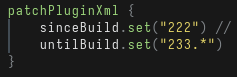
\includegraphics[width=7cm]{images/codegrits-wrong-version.png}
	\caption{Commande limittant les version utilisable d'IntelliJ}
	\label{codegrits-old-build-version}
\end{figure}

\begin{figure}
	\centering
	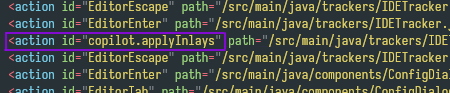
\includegraphics[width=10cm]{images/apply-inlay-action.png}
	\caption{Entrée du fichier \lstinline{ide_tracking.xml} référant à un évenement de complétion accéptée}
	\label{apply-inlay-action}
\end{figure}


\subsection{Modification}

Après avoir identifié les points manquants de l'extension CodeGRITS, il fallait maintenant trouver comment pallier à ce manque
en modifiant l'extension pour nos usages spécifiques.
À ce stade, il nous faut un moyens de tracker les moment ou l'extension Copilot viens suggerer du code au développeur, et que celui ci est visible
en grisé dans l'éditeur.

Plusieurs pistes on été envisagées, comme intercepter le traffic réseau entrant dans l'IDE, mais cela posait beaucoup de problème, nottament avec SSL.

Une approche beaucoup plus simple consistait à regarder les \emph{inlays} qui apparaissent dans l'éditeur,
c'est à dire les petits textes virtuels qui viennent donner des indications directement dans le viewport de l'éditeur de fichier,
comme par exemple le nom des paramêtre des fonctions, etc.
Ces \emph{inlays} sont gérés pour chaque fichier ouvert par un \emph{InlayModel}, auquel on peut attacher un listener afin de réagir
à la création / modification / destruction de ces inlays (voir Figure \ref{inlay-listener}).

Cependant, un fois cet accès acquit, il faut pouvoir récuperer les informations qui nous intéressent, ici le code proposé par GitHub Copilot.
Pour ce faire, il faut pouvoir détécter quel inlay nous intéresse, et récuperer les informations au bon endroit.

\begin{figure}
	\centering
	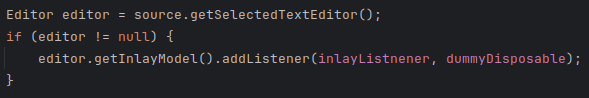
\includegraphics[width=10cm]{images/inlay-listener.png}
	\caption{Ajout d'un listener lors de l'ouverture d'un fichier}
	\label{inlay-listener}
\end{figure}


\subsubsection{Decompilation de Copilot}

GitHub Copilot n'étant pas du logiciel libre, il est impossible de regarder sont code de manière direct dur un depot publique, il faut donc trouver un autre moyens.
Heureusement, IntelliJ IDEA étant construit avec des technologies utilisant Java et la JVM, ses plugins aussi, il est donc possible de facilement décompiler l'extension afin de s'assurer de son fonctionnement.

Gâce à l'outil open source \emph{\href{https://java-decompiler.github.io/}{Java Decompiler}}, il est possible de retranscrir du bytecode executable par la JVM en code source java lisible (exemple Figure \ref{copilot-inlay-renderer}).
Sur l'image \ref{copilot-inlay-renderer}, on peut y voir une partie du code décompilé qui nous sera utile dans notre contexte: il s'agit du champ contenant le text qui s'affiche dans l'éditeur
quand Copilot veut nous suggerer quelque chose.

Comme on peut voir, il s'agit d'un champ privé, tout comme la classe qui l'abrite, mais java nous permet tout de même d'y acceder par des moyens détournés.

\begin{figure}
	\centering
	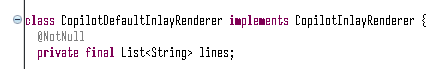
\includegraphics[width=10cm]{images/copilot-renderer-class.png}
	\caption{decompiled class of the inlay renderer in copilot's intellij plugin}
	\label{copilot-inlay-renderer}
\end{figure}


\subsubsection{Manipulation de la JVM}

Java est un language orienté objet, qui est compilé et éxécuté au sein d'un machine virtuelle, la JVM.
Les différentes visibilité des objets ne sont pas forcement garanties pendant l'execution du code comme elles le sont à la compilation.
Il est donc possible, en passant par des objets de la librairies standarde de Java, d'accèder à des champs privés de classes privés présentes
dans le contexte de la JVM courrante.

Dans l'adaptation de CodeGRITS que j'ai réalisé, je suis simplement allé chercher le champ \lstinline{lines} de l'objet renderer si il existait (voir \ref{getting-the-lines}).
Pour faire celà, Java propose dans la class \emph{Class<T>} un méthode permettant d'optenir un champ déclaré: \lstinline{getDeclaredField(String name)}.
Celle-ci nous permet d'intéragir avec le champ et de nottament modifier son accessibilité, et suite à quoi il est possible, peu importe la visibilité originale du champ,
d'acceder aux données qu'il renferme.

Ce procédé peut toutefois generer des exceptions d'accès illégal, d'où la présence d'un bloque \emph{try/catch} sur l'image \ref{getting-the-lines}.
Ettonement, pendant l'utilisation de cette modification, aucune de ces erreur ne m'as été renvoyée, il semblerai donc que cette methode fonctionne correctement.

\begin{figure}
	\centering
	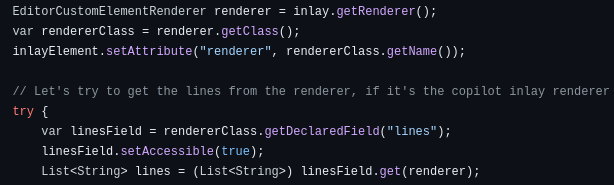
\includegraphics[width=15cm]{images/getting-the-lines.png}
	\caption{Récupération des données dans l'objet renderer de Copilot}
	\label{getting-the-lines}
\end{figure}

% -=+=-
% DATA
% -=+=-

\section{Analyse des données}

Lecture et structuration des données, création de graphs avec matplotlib, exploration de librairies plus intéractives (d3js, plotly)

\section{Soutenances de thèses (bonus)}

Vers la fin du mois de juin, j'ai pu assister a deux soutenances de thèses au sein du LaBRI.

\chapter{Git et Github (Internationalisation)}
\label{international}

TODO

\chapter{Bilan}
\label{bilan}

TODO


%----------------------------------------------------------------------------------------
%	THESIS CONTENT - APPENDICES
%----------------------------------------------------------------------------------------

\appendix % Cue to tell LaTeX that the following "chapters" are Appendices

% Include the appendices of the thesis as separate files from the Appendices folder
% Uncomment the lines as you write the Appendices

% \include{Appendices/AppendixA}
%\include{Appendices/AppendixB}
%\include{Appendices/AppendixC}

%----------------------------------------------------------------------------------------
%	BIBLIOGRAPHY
%----------------------------------------------------------------------------------------

\printbibliography[heading=bibintoc]

%----------------------------------------------------------------------------------------

\end{document}
